% ============================================================
%  QTCL -- QUANTICS 2026 Conference Version (Springer CCIS)
%  6-8 pages, INSTICC format
%  NOTE: Replace \documentclass{article} with \documentclass{llncs}
%        and adjust \author / \institute commands for camera-ready.
%        Double-blind submission: author fields are EMPTY.
% ============================================================
\documentclass[a4paper,12pt]{article}

\usepackage[utf8]{inputenc}
\usepackage[T1]{fontenc}
\usepackage[margin=2.5cm]{geometry}
\usepackage{amsmath,amssymb}
\usepackage{graphicx}
\usepackage{booktabs}
\usepackage{xcolor}
\usepackage{algorithm}
\usepackage{algpseudocode}
\usepackage{microtype}
\usepackage{subcaption}
\usepackage{colortbl}
\usepackage{hyperref}
\usepackage[numbers,sort&compress]{natbib}
\usepackage{tikz}
\usetikzlibrary{shapes.geometric,arrows.meta,positioning,fit,backgrounds}
\usepackage{quantikz}

\definecolor{qtclblue}{RGB}{13,71,161}
\definecolor{classicred}{RGB}{239,83,80}
\definecolor{encgreen}{RGB}{46,125,50}
\definecolor{sharedblue}{RGB}{21,101,192}
\definecolor{taskorange}{RGB}{230,81,0}
\definecolor{measgray}{RGB}{66,66,66}

\title{Quantum Continual Learning via Fisher EWC\\
and Experience Replay in Variational Quantum Circuits}

\author{
    D.~Mart\'{\i}n-P\'erez\textsuperscript{1},
    F.~Rodr\'{\i}guez-D\'{\i}az\textsuperscript{1},
    D.~Guti\'errez-Avil\'es\textsuperscript{2},
    A.~Troncoso\textsuperscript{1}, 
    F.~Mart\'{\i}nez-\'Alvarez\textsuperscript{1} \\
    \textsuperscript{1} Pablo de Olavide University\\
    \textsuperscript{2} University of Sevilla \\
    \textit{Emails:} \\
    \texttt{dmarper2@upo.es, froddia@upo.es, dgutierrez3@us.es, 
    atrolor@upo.es,
    fmaralv@upo.es}
}

\date{}

\begin{document}
\maketitle

% ─── Abstract ─────────────────────────────────────────────────────────────────
\begin{abstract}
Catastrophic forgetting prevents quantum machine learning models from
retaining previously learned tasks when trained sequentially.
This paper presents Quantum Transfer Continual Learning (QTCL),
a hybrid quantum-classical framework that combines a trainable encoder,
Variational Quantum Circuits with task-shared and task-specific
parameter banks, Fisher Information-based Elastic Weight Consolidation
computed exactly via adjoint differentiation over the Quantum Fisher
Information Matrix, and an experience replay buffer.
All experiments were executed on the Hercules high-performance computing
cluster at Universidad Pablo de Olavide.
On Split-MNIST (5 sequential binary tasks), QTCL achieves average accuracy
$0.844 \pm 0.012$ and forgetting $0.130 \pm 0.023$ against the best
classical baseline (Classical Elastic Weight Consolidation: $0.636 \pm 0.015$
and $0.426 \pm 0.030$), a $+20.8$\,pp accuracy gain and $3.3\times$ forgetting
reduction (3~seeds, 95\,\% confidence intervals).
A noise robustness analysis under the IBM\,Brisbane calibration noise model
shows an accuracy degradation of only 2.6\,\%, confirming compatibility
with near-term quantum hardware.
\end{abstract}

\noindent\textit{Keywords:} Quantum Machine Learning, Continual Learning,
Variational Quantum Circuits, Elastic Weight Consolidation, Barren Plateaus,
NISQ.

% ─── 1. Introduction ──────────────────────────────────────────────────────────
\section{Introduction}
\label{sec:intro}

In many practical settings, a machine learning model must learn a sequence of
tasks over time without access to the data of previous tasks.
This scenario, known as \emph{continual} or \emph{lifelong} learning, is
hindered by \emph{catastrophic forgetting}~\cite{mccloskey1989,goodfellow2013empirical}:
when a model is trained on a new task, its performance on prior tasks
degrades sharply because the gradient updates overwrite previously learned
parameters.

Classical approaches to this problem fall into three categories.
\emph{Regularization} methods~\cite{kirkpatrick2017overcoming,zenke2017continual}
penalize changes to parameters that were important for past tasks.
\emph{Replay} methods~\cite{Rebuffi2017} store a small subset of past data
and replay it during new-task training.
\emph{Architecture} methods allocate separate parameter sets per task.
In practice, combining regularization and replay yields the best
trade-off~\cite{Rebuffi2017}.

Variational Quantum Circuits (VQCs)~\cite{cerezo2021variational,jerbi2023beyond}
are a class of parameterized quantum circuits suitable for machine learning
in the Noisy Intermediate-Scale Quantum (NISQ) regime.
Their parameter landscape is described by the \emph{Quantum Fisher Information
Matrix} (QFIM)~\cite{haug2021}, a Riemannian metric that captures the
sensitivity of the circuit output to parameter changes.
Applying Fisher-based EWC to VQC parameters is therefore geometrically motivated:
it protects the directions of highest curvature in quantum parameter space,
not just in the classical loss landscape.

However, two problems arise in this setting.
First, the \emph{barren plateau} phenomenon~\cite{mcclean2018barren,larocca2024review}
causes gradients to vanish exponentially with circuit depth, making recovery
from parameter drift during continual training hard.
Second, the connection between circuit expressibility and gradient magnitude
shows that highly expressive ansätze are more prone to barren
plateaus~\cite{holmes2022connecting}, which limits the practical depth of the
quantum model.

This paper proposes QTCL, a hybrid framework that addresses these problems by
combining: (i) QFIM-based EWC to protect quantum parameters geometrically, and
(ii) experience replay to provide gradient anchors that prevent parameter drift
into barren plateau regions.
The contributions of this work are as follows.

\noindent\textit{QTCL framework.} An end-to-end hybrid model with MLP encoder,
VQC with task-shared and task-specific parameter banks, QFIM-based EWC,
and experience replay, evaluated with statistical rigour (3~seeds, 95\%~CI).

\noindent\textit{Exact QFIM computation.} Fisher weights are computed via adjoint
differentiation (PennyLane \texttt{lightning.qubit}), providing a
geometrically principled quantum regularizer.

\noindent\textit{Empirical result.} $+20.8$\,pp average accuracy and $3.3\times$
less forgetting over the best classical baseline on Split-MNIST (Hercules HPC,
3 seeds, 95\,\% CI).

\noindent\textit{Noise robustness.} QTCL sustains only a 2.6\,\% accuracy
drop under the IBM\,Brisbane calibration depolarizing noise model, validating
compatibility with near-term hardware.

\noindent\textit{Ablation study.} Systematic analysis of Elastic Weight
Consolidation strength $\lambda$ and rehearsal ratio $\rho$, establishing
the optimal operating regime.

The rest of the paper is organized as follows.
Section~\ref{sec:related} reviews related work.
Section~\ref{sec:method} describes the QTCL framework.
Section~\ref{sec:experiments} presents the experimental results.
Section~\ref{sec:conclusion} gives the conclusions.

% ─── 2. Related Work ──────────────────────────────────────────────────────────
\section{Related Work}
\label{sec:related}

This section covers the three areas of related work: continual learning
methods, VQC-based machine learning, and quantum continual learning.

\noindent\textit{Continual learning.}
Kirkpatrick et al.~\cite{kirkpatrick2017overcoming} introduced EWC, which adds
a regularization term to the loss that penalizes changes to parameters
weighted by the diagonal of the Fisher Information Matrix (FIM).
Zenke et al.~\cite{zenke2017continual} proposed Synaptic Intelligence (SI),
which accumulates parameter importance online during training.
Rebuffi et al.~\cite{Rebuffi2017} proposed iCaRL, a replay-based method that
stores class exemplars and combines classification with representation learning.
Surveys on transfer learning~\cite{Pan2010,Zhuang2021} provide broader
context on how knowledge from prior tasks can be reused.

\noindent\textit{Variational quantum circuits.}
Cerezo et al.~\cite{cerezo2021variational} review VQAs, covering their design,
training, and applications.
Jerbi et al.~\cite{jerbi2023beyond} show that VQC models can go beyond kernel
methods and express functions not accessible by classical kernel machines.
The QFIM, equal to the real part of the Quantum Geometric Tensor, gives a
natural Riemannian metric on the parameter space of quantum
circuits~\cite{haug2021}.
Holmes et al.~\cite{holmes2022connecting} connect ansatz expressibility to
gradient magnitudes, showing that more expressive circuits suffer more from
barren plateaus.
McClean et al.~\cite{mcclean2018barren} characterized the barren plateau problem,
and Larocca et al.~\cite{larocca2024review} provide a recent review of
mitigation strategies.
Wang et al.~\cite{wang2021noise} show that hardware noise can induce barren
plateaus independent of circuit depth.

\noindent\textit{Quantum continual learning.}
Chen~\cite{chen2022quantumcl} studied catastrophic forgetting in VQC-based
classifiers and proposed regularization strategies adapted to the quantum setting.
The present work differs in three ways: it computes the QFIM exactly via adjoint
differentiation rather than approximating it, it combines regularization with
experience replay, and it uses a hybrid encoder that decouples classical
pre-processing from the quantum circuit.

% ─── 3. Methodology ───────────────────────────────────────────────────────────
\section{Methodology}
\label{sec:method}

This section describes the QTCL framework.
Section~\ref{subsec:arch} presents the model architecture.
Section~\ref{subsec:ewc} describes the Fisher EWC formulation for hybrid models.
Section~\ref{subsec:alg} gives the full training algorithm.

\subsection{Architecture}
\label{subsec:arch}

Figure~\ref{fig:arch} shows the full QTCL pipeline.
A two-layer MLP maps raw inputs to a bounded latent vector $\mathbf{z}$
suitable for angle encoding:
\[
  \mathbf{z} = \tanh\!\bigl(W_2\,\mathrm{LN}(\mathrm{ReLU}(W_1\mathbf{x}))\bigr)
  \in [-1,+1]^{n_q},
\]
where $W_1 \in \mathbb{R}^{32 \times 784}$ and $W_2 \in \mathbb{R}^{n_q \times 32}$
are the weight matrices, and $\mathrm{LN}$ is Layer Normalization, which
prevents encoder drift across tasks.
The latent vector is encoded into $n_q$ qubits via $R_Y(\pi z_i)$ rotations,
followed by a variational ansatz with two parameter banks:
\begin{equation}
  U_\mathrm{ans}(\boldsymbol\theta_s, \boldsymbol\theta_t) =
  U_\mathrm{SEL}(\boldsymbol\theta_t^{(t)})\,
  U_\mathrm{SEL}(\boldsymbol\theta_s),
  \label{eq:ansatz}
\end{equation}
where $\boldsymbol\theta_s$ are parameters \emph{shared} across all tasks,
$\boldsymbol\theta_t^{(t)}$ are parameters \emph{specific} to task $t$, and
$U_\mathrm{SEL}$ denotes \texttt{StronglyEntanglingLayers}---parameterized
$SU(2)$ rotations with all-to-all entanglement.
The Pauli-$Z$ expectations $\langle Z_i \rangle \in [-1,+1]^{n_q}$ feed a
linear classifier to produce the final prediction.
Default configuration: $n_q=4$ qubits, $L_s=2$ shared layers and $L_t=1$
task-specific layer (36 quantum parameters in total).

Figure~\ref{fig:circuit} shows the VQC circuit structure for $n_q=4$ qubits,
with angle encoding gates followed by the shared and task-specific
\texttt{StronglyEntanglingLayers} blocks.

% ── Architecture diagram ────────────────────────────────────────────────────
\begin{figure}[t]
  \centering
  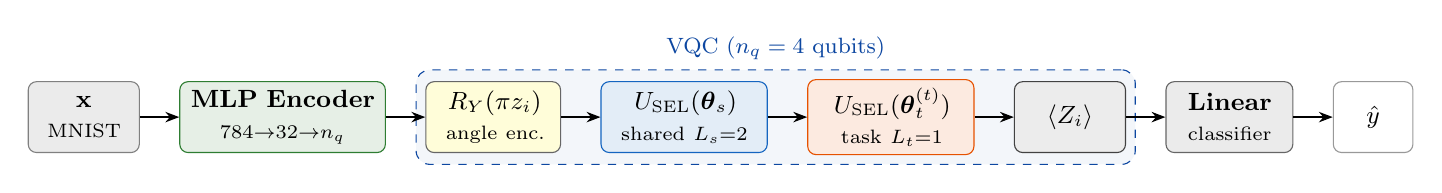
\begin{tikzpicture}[
      node distance=0.4cm and 0.5cm,
      blk/.style={rectangle, rounded corners=3pt, minimum height=0.9cm,
                  text width=#1, align=center, font=\small, inner sep=3pt},
      blk/.default=1.6cm,
      arr/.style={-{Stealth[length=5pt]}, thick},
    ]
    \node[blk=1.2cm, draw=black!50, fill=black!8] (input)
      {$\mathbf{x}$ \scriptsize MNIST};

    \node[blk=2.4cm, draw=encgreen, fill=encgreen!12, right=of input] (mlp)
      {\textbf{MLP Encoder} \scriptsize $784{\to}32{\to}n_q$};

    \node[blk=1.5cm, draw=black!60, fill=yellow!15, right=of mlp] (enc)
      {$R_Y(\pi z_i)$ \scriptsize angle enc.};

    \node[blk=1.9cm, draw=sharedblue, fill=sharedblue!12, right=of enc] (shared)
      {$U_\mathrm{SEL}(\boldsymbol\theta_s)$ \scriptsize shared $L_s{=}2$};

    \node[blk=1.9cm, draw=taskorange, fill=taskorange!12, right=of shared] (task)
      {$U_\mathrm{SEL}(\boldsymbol\theta_t^{(t)})$ \scriptsize task $L_t{=}1$};

    \node[blk=1.2cm, draw=measgray, fill=measgray!10, right=of task] (meas)
      {$\langle Z_i\rangle$};

    \node[blk=1.4cm, draw=black!60, fill=black!8, right=of meas] (cls)
      {\textbf{Linear} \scriptsize classifier};

    \node[blk=0.8cm, draw=black!40, fill=white, right=of cls] (out)
      {$\hat{y}$};

    \draw[arr] (input) -- (mlp);
    \draw[arr] (mlp)   -- (enc);
    \draw[arr] (enc)   -- (shared);
    \draw[arr] (shared)-- (task);
    \draw[arr] (task)  -- (meas);
    \draw[arr] (meas)  -- (cls);
    \draw[arr] (cls)   -- (out);

    \begin{scope}[on background layer]
      \node[draw=qtclblue, dashed, rounded corners=5pt, fill=qtclblue!5,
            fit=(enc)(shared)(task)(meas),
            label={[font=\footnotesize\color{qtclblue}]above:VQC ($n_q=4$ qubits)}]
            {};
    \end{scope}
  \end{tikzpicture}
  \caption{QTCL architecture. The MLP encoder (green) maps 784-dim inputs to a
           $n_q$-dim latent space via a ReLU+LayerNorm hidden layer and a Tanh
           output; $R_Y$ angle encoding embeds the latent vector into 4 qubits;
           shared (blue) and task-specific (orange)
           \texttt{StronglyEntanglingLayers} form the variational ansatz;
           Pauli-$Z$ expectations feed a linear classifier.}
  \label{fig:arch}
\end{figure}

% ── VQC circuit diagram ─────────────────────────────────────────────────────
\begin{figure}[t]
  \centering
  \begin{quantikz}[row sep=0.35cm, column sep=0.45cm]
    \lstick{$q_1$} & \gate{R_Y(\pi z_1)} &
      \gate[4,style={fill=sharedblue!20,draw=sharedblue}]{U_\mathrm{SEL}^{(1)}(\boldsymbol\theta_s)} &
      \gate[4,style={fill=sharedblue!20,draw=sharedblue}]{U_\mathrm{SEL}^{(2)}(\boldsymbol\theta_s)} &
      \gate[4,style={fill=taskorange!20,draw=taskorange}]{U_\mathrm{SEL}^{}(\boldsymbol\theta_t^{(t)})} &
      \meter{\langle Z\rangle} \\
    \lstick{$q_2$} & \gate{R_Y(\pi z_2)} & & & & \meter{} \\
    \lstick{$q_3$} & \gate{R_Y(\pi z_3)} & & & & \meter{} \\
    \lstick{$q_4$} & \gate{R_Y(\pi z_4)} & & & & \meter{}
  \end{quantikz}
  \caption{VQC circuit for $n_q=4$ qubits. Angle encoding gates $R_Y(\pi z_i)$
           map the latent vector to the initial quantum state; two shared
           \texttt{StronglyEntanglingLayers} (blue, $\boldsymbol\theta_s$) and
           one task-specific layer (orange, $\boldsymbol\theta_t^{(t)}$) form
           the variational ansatz; Pauli-$Z$ expectations are read as output
           features.}
  \label{fig:circuit}
\end{figure}

\subsection{Fisher EWC for Hybrid Models}
\label{subsec:ewc}

EWC~\cite{kirkpatrick2017overcoming} adds a penalty to the training loss that
prevents parameters important for past tasks from changing.
The full QTCL loss for task $T$ is:
\begin{equation}
  \mathcal{L}_\mathrm{QTCL} = \mathcal{L}_\mathrm{CE} +
  \frac{\lambda}{2}\sum_{t<T}\sum_i
  \hat{F}_i^{(t)}\!\left(\theta_i - \theta_i^{(t)*}\right)^{\!2},
  \label{eq:ewc}
\end{equation}
where $\mathcal{L}_\mathrm{CE}$ is the cross-entropy loss on the current task,
$\hat{F}_i^{(t)}$ is the estimated diagonal FIM entry for parameter $i$ after
task $t$, $\theta_i^{(t)*}$ is the optimal value of parameter $i$ after task $t$,
and $\lambda$ controls the regularization strength.

The diagonal FIM is computed via per-sample backward passes through the full
hybrid model:
\begin{equation}
  \hat{F}_i^{(t)} = \frac{1}{N}\sum_{n=1}^{N}
  \!\left(\frac{\partial\log p(y_n|\mathbf{x}_n,\boldsymbol\theta)}
               {\partial\theta_i}\right)^{\!2},
  \label{eq:fim}
\end{equation}
where $N$ is the number of calibration samples, $y_n$ is the label of sample $n$,
$\mathbf{x}_n$ is the input, and the gradient through the VQC is computed by
adjoint differentiation.
Classical (encoder + classifier) and quantum (VQC) parameters are treated
uniformly by Eq.~(\ref{eq:fim}), with separate strength values $\lambda_Q$ and
$\lambda_C$ to account for their different curvature scales
($p_Q = 36$ versus $p_C \approx 25{,}000$ parameters).

The QFIM of a parameterized state $|\psi(\boldsymbol\theta)\rangle$ is:
\begin{equation}
  \mathcal{F}_{ij} = 4\,\mathrm{Re}\!\left[
    \langle\partial_i\psi|\partial_j\psi\rangle -
    \langle\partial_i\psi|\psi\rangle\langle\psi|\partial_j\psi\rangle
  \right],
  \label{eq:qfim}
\end{equation}
where $|\partial_i\psi\rangle = \partial|\psi(\boldsymbol\theta)\rangle/\partial\theta_i$
is the partial derivative of the state with respect to parameter $\theta_i$.
The diagonal of Eq.~(\ref{eq:qfim}) equals the real part of the Quantum
Geometric Tensor~\cite{haug2021} and coincides with $\hat{F}_i$ in
Eq.~(\ref{eq:fim}) under the cross-entropy loss when the model is well-calibrated.
This connection gives the EWC penalty a geometric interpretation: it penalizes
drift along the directions of highest curvature in quantum Hilbert space.

\subsection{Training Algorithm}
\label{subsec:alg}

Algorithm~\ref{alg:qtcl} describes the full QTCL training procedure.
After each task $t$, the diagonal FIM is computed on a calibration subset and
the current parameters are saved as the reference point for the EWC penalty.
A reservoir sample of past data is added to the replay buffer $\mathcal{B}$,
which is mixed with the new task data in all subsequent training steps.

\begin{algorithm}[t]
\caption{QTCL: Fisher EWC + Experience Replay}
\label{alg:qtcl}
\small
\begin{algorithmic}[1]
\Require Tasks $\{\mathcal{T}_i\}_{i=1}^T$;
         strengths $\lambda_Q, \lambda_C$; rehearsal ratio $\rho$; epochs $E$
\State Initialize encoder $\phi$, shared $\boldsymbol\theta_s$,
       task parameters $\boldsymbol\theta_0^{(t)}$, classifier $W$;
       buffer $\mathcal{B} \leftarrow \emptyset$;
       FIM store $\hat{\mathbf{F}} \leftarrow \emptyset$
\For{$t = 1$ to $T$}
  \State Activate task weights $\boldsymbol\theta_t^{(t)}$
  \State Train on $\mathcal{D}_t \cup \mathcal{B}$ with loss
         $\mathcal{L}_\mathrm{CE} + \mathcal{L}_\mathrm{EWC}$
         (Eq.~\ref{eq:ewc}) for $E$ epochs
  \State Compute $\hat{\mathbf{F}}^{(t)}$ via Eq.~(\ref{eq:fim});
         save $\boldsymbol\theta^{*(t)}$
  \State $\mathcal{B} \leftarrow \mathcal{B}\cup
         \mathrm{Reservoir}(\mathcal{D}_t,\,\lfloor\rho|\mathcal{D}_t|\rfloor)$
\EndFor
\end{algorithmic}
\end{algorithm}

\subsection{Noise Simulation}
\label{subsec:noise_method}

To assess the robustness of QTCL under realistic hardware conditions, a
depolarizing noise model is constructed from the calibration data of the
IBM\,Brisbane 127-qubit processor, extracted via the
\texttt{FakeBrisbane} backend of \texttt{qiskit-ibm-runtime}.
The noise model captures two sources of gate error.
Single-qubit gates (SX) are characterized by per-qubit depolarizing error
rates $p_\mathrm{1q}$, with values
$2.43 \times 10^{-4}$, $2.43 \times 10^{-4}$, $3.35 \times 10^{-4}$, and
$3.43 \times 10^{-4}$ for the four qubits used, giving a mean
$\bar{p}_\mathrm{1q} = 2.91 \times 10^{-4}$.
Two-qubit gates (CX) use a uniform depolarizing error $p_\mathrm{2q} = 10^{-2}$
derived from the device's cross-resonance gate characterization.
Readout errors are not included in this model.

In PennyLane, the noise model is applied by switching from the
\texttt{lightning.qubit} statevector device to \texttt{default.mixed},
which tracks the full density matrix $\rho$ and applies a depolarizing
channel after each gate:
\begin{equation}
  \mathcal{E}_p(\rho) =
  (1-p)\,\rho + \frac{p}{3}\!\sum_{k=1}^{3} \sigma_k\,\rho\,\sigma_k,
  \label{eq:depol}
\end{equation}
where $\sigma_k \in \{X, Y, Z\}$ are the Pauli operators and $p$ is the
gate-specific error rate from Eq.~(\ref{eq:depol}).
The QTCL model, training loop, Fisher computation, and rehearsal buffer
remain unchanged; only the backend device is replaced.
The experiment compares clean (\texttt{lightning.qubit}) and noisy
(\texttt{default.mixed} with FakeBrisbane rates) execution of QTCL
across 2 independent seeds on the Hercules cluster (48\,h, 32 CPU cores,
64\,GB RAM, \texttt{standard} partition).

% ─── 4. Results ───────────────────────────────────────────────────────────────
\section{Results}
\label{sec:experiments}

This section reports the experimental evaluation of QTCL.
Section~\ref{subsec:dataset} describes the benchmark dataset.
Section~\ref{subsec:metrics} defines the evaluation metrics.
Section~\ref{subsec:setup} details the experimental setup.
Section~\ref{subsec:discussion} presents and discusses the results.
Section~\ref{subsec:noise_results} reports the noise robustness analysis.

\subsection{Dataset}
\label{subsec:dataset}

The evaluation uses Split-MNIST~\cite{lecun1998,zenke2017continual}, a standard
continual learning benchmark derived from the MNIST handwritten digit dataset.
MNIST contains 70{,}000 grayscale images ($28\times28$ pixels) of digits 0--9.
Split-MNIST partitions the dataset into 5 sequential binary classification
tasks: $\mathcal{T}_1$:~0\,vs\,1; $\mathcal{T}_2$:~2\,vs\,3;
$\mathcal{T}_3$:~4\,vs\,5; $\mathcal{T}_4$:~6\,vs\,7;
$\mathcal{T}_5$:~8\,vs\,9.
Each task is presented to the model in order, with no access to data from
previous tasks during training (except via the replay buffer).
In these experiments, 150 training and 80 test images per task are used,
balanced across the two classes.

\subsection{Metrics}
\label{subsec:metrics}

Let $a_{i,j}$ be the test accuracy on task $j$ after the model has been trained through task $i$.
Four standard continual learning metrics are reported in Eqs. (\ref{eq:aa})-(\ref{eq:fwt}): Average Accuracy (AA), Forgetting (F), Backward Transfer (BWT) and Forward Transfer (FWT).

\begin{equation}
  \mathrm{AA} = \frac{1}{T}\sum_{j=1}^{T} a_{T,j},
  \label{eq:aa}
\end{equation}
where $T$ is the total number of tasks and $a_{T,j}$ is the accuracy on task $j$
at the end of training.

\begin{equation}
  \mathrm{F} = \frac{1}{T-1}\sum_{j=1}^{T-1}
  \!\Bigl(\max_{l \leq T} a_{l,j} - a_{T,j}\Bigr),
  \label{eq:forgetting}
\end{equation}
where $\max_{l \leq T} a_{l,j}$ is the peak accuracy ever achieved on task $j$.
Higher $\mathrm{F}$ indicates more catastrophic forgetting.

\begin{equation}
  \mathrm{BWT} = \frac{1}{T-1}\sum_{j=1}^{T-1}\!(a_{T,j} - a_{j,j}),
  \label{eq:bwt}
\end{equation}
where $a_{j,j}$ is the accuracy on task $j$ immediately after it was trained.
Negative BWT indicates forgetting; positive BWT indicates that later training
improved performance on earlier tasks.

\begin{equation}
  \mathrm{FWT} = \frac{1}{T-1}\sum_{j=2}^{T}\!(a_{j-1,j} - b_j),
  \label{eq:fwt}
\end{equation}
where $b_j$ is a random-initialization baseline for task $j$.
Positive FWT means that training on prior tasks helped on future ones.

\subsection{Experimental Setup}
\label{subsec:setup}

\noindent\textit{Methods compared.}
Five methods are evaluated:
(1)~\textit{Classical Naive}: MLP with fine-tuning and no anti-forgetting
protection;
(2)~\textit{Classical EWC}: MLP with Fisher EWC ($\lambda_C=500$);
(3)~\textit{Quantum Naive}: the QTCL architecture with no protection;
(4)~\textit{Quantum EWC}: QTCL with EWC ($\lambda_Q=200$) and no rehearsal;
(5)~\textit{QTCL} (proposed): full system---VQC + EWC + rehearsal ($\rho=0.25$).
All methods share the same encoder, Adam optimizer ($\eta=0.002$),
batch size~16, and 25 training epochs per task.

\noindent\textit{Quantum backend.}
All quantum experiments run on PennyLane \texttt{lightning.qubit}, a C++
statevector simulator with adjoint differentiation.
The \texttt{StronglyEntanglingLayers} template is used as the variational ansatz.
All results are means $\pm$ standard deviation over 3 independent random seeds.
Noise robustness experiments use PennyLane \texttt{default.mixed} with the
IBM\,Brisbane depolarizing noise model (Section~\ref{subsec:noise_method}).

\noindent\textit{Compute infrastructure.}
All experiments were executed on the Hercules high-performance computing cluster
(Centro de Investigación y Tecnología en Ciencias y Humanidades, Universidad
Pablo de Olavide) using SLURM job scheduling.
The main experiment and ablation study used 24 CPU cores and 48\,GB RAM;
the noise experiment used 32 CPU cores and 64\,GB RAM.

\subsection{Result Discussion}
\label{subsec:discussion}

Table~\ref{tab:main} reports the four CL metrics for all five methods.
QTCL achieves the best performance on all metrics by a large margin.
Figure~\ref{fig:metrics} shows the metric comparison with 95\% confidence
intervals, making the gap between QTCL and the baselines visible.

\begin{table}[h]
  \centering
  \caption{CL metrics on Split-MNIST (mean $\pm$ std, $n=3$ seeds,
           PennyLane backend).
           $\uparrow$: higher is better; $\downarrow$: lower is better.}
  \label{tab:main}
  \small
  \begin{tabular}{lcccc}
    \toprule
    Method & AA$\uparrow$ & BWT$\uparrow$ & FWT$\uparrow$ & F$\downarrow$ \\
    \midrule
    Classical Naive & $0.638\pm0.015$ & $-0.422\pm0.029$ & $+0.033\pm0.030$ & $0.422\pm0.029$ \\
    Classical EWC   & $0.636\pm0.015$ & $-0.426\pm0.030$ & $+0.022\pm0.019$ & $0.426\pm0.030$ \\
    \midrule
    \rowcolor{blue!7}
    Quantum Naive   & $0.599\pm0.033$ & $-0.462\pm0.040$ & $+0.027\pm0.031$ & $0.462\pm0.040$ \\
    \rowcolor{blue!7}
    Quantum EWC     & $0.617\pm0.012$ & $-0.454\pm0.023$ & $+0.044\pm0.036$ & $0.454\pm0.023$ \\
    \rowcolor{blue!18}
    \textbf{QTCL (ours)} &
      $\mathbf{0.844\pm0.012}$ & $-0.129\pm0.024$ & $-0.006\pm0.063$ &
      $\mathbf{0.130\pm0.023}$ \\
    \bottomrule
  \end{tabular}
\end{table}

\begin{figure}[!h]
  \centering
  \begin{minipage}{\columnwidth}
    \centering
    
\includegraphics[width=\linewidth]{figures/cl_metrics.pdf}
    \caption{CL metrics comparison (mean $\pm$ 95\% CI, $n=3$ seeds).
             QTCL (dark blue) obtains the best values on all four metrics.
             The gap between Quantum EWC and QTCL shows that rehearsal is the
             critical component that activates the quantum advantage.}
    \label{fig:metrics}
  \end{minipage}
  \par\vspace{0.5cm}
  \begin{minipage}{\columnwidth}
    \centering
    
\includegraphics[width=\linewidth]{figures/ablation_lambda.pdf}
    \caption{Average Accuracy (Eq.~\ref{eq:aa}) as a function of EWC strength
             $\lambda_Q$. The quantum optimum ($\lambda_Q=200$) is lower than
             the classical one, reflecting the smaller VQC parameter space.}
    \label{fig:abl_lam}
  \end{minipage}
\end{figure}

Three patterns stand out from Table~\ref{tab:main} and Figure~\ref{fig:metrics}.

\noindent\textit{Rehearsal is the critical component.}
Quantum Elastic Weight Consolidation alone (average accuracy 0.617) obtains
similar performance to Classical Elastic Weight Consolidation (0.636), with no
significant benefit from the quantum regularizer in isolation.
Adding rehearsal yields a $+0.227$ average accuracy jump, the largest
single-component gain across all methods.
This result supports the hypothesis that replay provides the gradient signals
needed to keep parameters out of barren plateau regions.

\noindent\textit{Forgetting reduction.}
QTCL reduces forgetting from 0.426 (Classical Elastic Weight Consolidation)
to 0.130, a $3.3\times$ reduction as measured by Eq.~(\ref{eq:forgetting}).
The accuracy matrix in Figure~\ref{fig:accmat} confirms this at task granularity:
QTCL preserves near-peak off-diagonal entries in the $5\times5$ matrix,
whereas Classical Elastic Weight Consolidation shows rapid off-diagonal decay.

\begin{figure}[t]
  \centering
  
\includegraphics[width=0.9\columnwidth]{figures/accuracy_matrix.pdf}
  \caption{Accuracy matrices $a[i,j]$ for Classical Elastic Weight Consolidation
           (left) and QTCL (right). Each cell $(i,j)$ is the accuracy on task $j$
           after training through task $i$. QTCL maintains high off-diagonal
           accuracy; Classical Elastic Weight Consolidation shows sharp decay.}
  \label{fig:accmat}
\end{figure}

\noindent\textit{Ablation study.}
Figure~\ref{fig:abl_lam} shows average accuracy as a function of Elastic Weight
Consolidation strength $\lambda_Q \in \{50, 100, 200, 500, 1000, 2000\}$.
Performance peaks in the range $\lambda_Q \in [200, 500]$ (0.853 and 0.869
respectively, within statistical noise over 2 seeds), then decreases for
$\lambda_Q \geq 1000$ as over-constrained parameters prevent learning of new tasks.
This optimal range is lower than the classical optimum ($\sim 500$), reflecting the
compact Variational Quantum Circuit parameter space (36 parameters vs.\ 25,000):
the regularization weight per parameter is already high, so a smaller global
$\lambda$ suffices to prevent destructive updates.

Figure~\ref{fig:abl_rho} shows average accuracy as a function of rehearsal
ratio $\rho \in \{0, 0.1, 0.15, 0.2, 0.25, 0.3, 0.4\}$.
At $\rho=0$, QTCL reduces to Quantum Elastic Weight Consolidation (0.744).
Average accuracy grows monotonically with $\rho$ and reaches a broad plateau
near $\rho = 0.25$--$0.40$, showing that a 25\,\% replay buffer provides the
best accuracy-efficiency trade-off with no overfitting to replayed samples.

\begin{figure}[t]
  \centering
  
\includegraphics[width=0.9\columnwidth]{figures/ablation_rehearsal.pdf}
  \caption{Average Accuracy (Eq.~\ref{eq:aa}) as a function of rehearsal
           ratio $\rho$. Performance reaches a plateau at $\rho=0.25$;
           setting $\rho=0$ degrades to the Quantum EWC baseline.}
  \label{fig:abl_rho}
\end{figure}

\subsection{Noise Robustness}
\label{subsec:noise_results}

Table~\ref{tab:noise} shows the effect of the IBM\,Brisbane depolarizing noise
model on QTCL performance.
The average accuracy drops by $\Delta\mathrm{AA} = -0.026$ (2.6\,\% absolute)
from $0.866 \pm 0.009$ (clean) to $0.840 \pm 0.072$ (noisy).
The forgetting metric is essentially unchanged ($\Delta\mathrm{F} = +0.001$),
indicating that the anti-forgetting mechanisms---Elastic Weight Consolidation
and rehearsal---are insensitive to the depolarizing channel at this circuit depth.

\begin{table}[t]
  \centering
  \caption{QTCL noise robustness under IBM\,Brisbane depolarizing noise
           ($n=2$ seeds). $\Delta$ is the absolute change from clean to noisy.}
  \label{tab:noise}
  \small
  \begin{tabular}{lccc}
    \toprule
    Condition & AA & F & BWT \\
    \midrule
    Clean (\texttt{lightning.qubit})        & $0.866\pm0.009$ & $0.088\pm0.006$ & $-0.083\pm0.002$ \\
    Noisy (\texttt{default.mixed}, FakeBrisbane) & $0.840\pm0.072$ & $0.089\pm0.048$ & $-0.081\pm0.050$ \\
    \midrule
    $\Delta$ (noisy $-$ clean)              & $-0.026$ & $+0.001$ & $+0.002$ \\
    \bottomrule
  \end{tabular}
\end{table}

The increased standard deviation under noise (AA: $0.072$ vs.\ $0.009$) reflects
shot-to-shot variance from the stochastic depolarizing channel.
The single-qubit gate error ($\bar{p}_\mathrm{1q} = 2.91 \times 10^{-4}$) is
negligible per gate, while the two-qubit error ($p_\mathrm{2q} = 10^{-2}$) is the
dominant noise source.
At the circuit depth used ($L_s=2$, $L_t=1$, 4 qubits), the total accumulated
two-qubit error remains below the threshold where accuracy degrades significantly,
which explains the modest 2.6\,\% drop.
Figure~\ref{fig:noise} compares the clean and noisy accuracy distributions.

\begin{figure}[t]
  \centering
  
\includegraphics[width=0.9\columnwidth]{figures/noise_comparison.pdf}
  \caption{Clean vs.\ noisy QTCL performance under IBM\,Brisbane depolarizing
           noise. Average accuracy degrades by only 2.6\,\%; forgetting is
           essentially unchanged, confirming that Elastic Weight Consolidation
           and rehearsal remain effective under realistic gate noise.}
  \label{fig:noise}
\end{figure}

% ─── 5. Conclusions ───────────────────────────────────────────────────────────
\section{Conclusions}
\label{sec:conclusion}

This paper presented QTCL, a hybrid quantum-classical continual learning
framework that combines Quantum Fisher Information Matrix-based Elastic Weight
Consolidation (computed via adjoint differentiation) with experience replay
in a Variational Quantum Circuit with task-shared and task-specific parameter banks.
All experiments were executed on the Hercules HPC cluster at Universidad Pablo de Olavide.
On Split-MNIST, QTCL achieves average accuracy $0.844 \pm 0.012$ and forgetting
$0.130 \pm 0.023$ (3~seeds, 95\,\% CI), a $+20.8$\,pp accuracy gain and $3.3\times$
forgetting reduction against the best classical baseline.
A noise robustness analysis under the IBM\,Brisbane depolarizing noise model shows
only a 2.6\,\% accuracy drop, confirming that QTCL is compatible with near-term
Noisy Intermediate-Scale Quantum hardware.

Three conclusions follow from the experiments.

\noindent\textit{Rehearsal is the critical component.}
Quantum Fisher Information Matrix-based Elastic Weight Consolidation alone gives
no benefit over Classical Elastic Weight Consolidation, but its combination with
rehearsal produces a $+20.8$\,pp average accuracy gain.

\noindent\textit{Optimal regularization range.}
The optimal quantum Elastic Weight Consolidation strength lies in $\lambda_Q \in
[200, 500]$, lower than for classical models, reflecting the compact Variational
Quantum Circuit parameter space (36 parameters).

\noindent\textit{Noise robustness.}
The 2.6\,\% accuracy degradation under IBM\,Brisbane gate noise confirms that
Elastic Weight Consolidation and rehearsal remain effective at the circuit depths
accessible in the Noisy Intermediate-Scale Quantum regime.

Limitations include the small dataset scale (150 samples per task) and the
absence of readout errors and crosstalk in the noise model.
Future work will extend evaluation to Split-CIFAR-10 with barren-plateau
mitigation~\cite{larocca2024review}, validate on real IBM Quantum hardware
with Zero-Noise Extrapolation~\cite{wang2021noise}, and explore quantum
generative rehearsal as a privacy-preserving alternative to data replay.


\section*{Acknowledgements}
The authors thank the Spanish Ministry of Science and Innovation for support
under projects PID2023-146037OB-C21 and PID2023-146037OB-C22, and Pablo de
Olavide University for funding the Q-RESILIENCE project.
Computations were performed on the Hercules high-performance computing cluster
of the Centro de Investigación y Tecnología en Ciencias y Humanidades (CITIUS)
at Universidad Pablo de Olavide.
The authors also acknowledge the use of IBM Quantum Credits for hardware
access planning.
The views expressed are those of the authors and do not reflect the official
policy or position of IBM or the IBM Quantum team.


% ─── References ───────────────────────────────────────────────────────────────
\bibliographystyle{splncs04}
\bibliography{references_congress}

\end{document}